\chapter{Supplementary SPADE Diagnostics and Sensitivity Tests}
\label{app:spade_diagnostics}

This appendix gives the numerical diagnostics and provisional sensitivity tests that support Chapter~\ref{ch:exoplanet_experiment}.  Keeping these details here makes the analysis reproducible without interrupting the main channel-model argument.  The assumed workbench parameters are not experimental measurements.

\section{Channel Classification and Parameter Sources}

Table~\ref{tab:spade_channel_sequence} records the role and source of every parameter in the sequential model.  ``Conditional'' means that a result can be calculated only after the relevant parameters have been fixed by an external calibration or stated assumption.

\begin{table}[htbp]
    \centering
    \caption{Experiment-specific channel sequence, parameter sources, and possible information effects.}
    \label{tab:spade_channel_sequence}
    \begin{tabularx}{\textwidth}{p{3cm} p{5cm} X}
        \toprule
        \rowcolor{gray!5} \textbf{Stage}  & \textbf{Parameter source}                                               & \textbf{Information effect}                                            \\
        \midrule
        \rowcolor{gray!15} \multicolumn{3}{l}{\textbf{Quantum preparation and channels}}                                                                                                     \\
        \midrule
        Bright / \newline faint mixture   & $d_a,\epsilon$ programmed. Source form assumed                          & Defines the source-state QFI                                           \\
        Survival / \newline erasure       & $\eta$ unidentifiable without launched flux                             & Can change QFI per launched photon                                     \\
        Alignment / \newline displacement & Effective offset fitted. Physical sorter offset not isolated            & Fixed unitary preserves state QFI but can reduce fixed-measurement CFI \\
        Dephasing                         & Cannot be identified. Provisional visibility used only in the workbench & Can reduce state QFI. Immediate HG populations remain unchanged        \\
        Coherent HG mixing                & Provisional angle and phase used only in the workbench                  & Fixed unitary preserves QFI but redistributes measurement CFI          \\
        Modal transmission                & Provisional transmissions used only in the workbench                    & Can reduce accessible QFI and CFI                                      \\
        Accessible-mode reduction         & Selected HG subspace specified. Complement outcome unrecorded           & Can reduce state QFI while keeping the failure probability             \\
        \midrule
        \rowcolor{gray!15} \multicolumn{3}{l}{\textbf{Quantum measurement}}                                                                                                                  \\
        \midrule
        SPADE                             & Modal basis specified. Full outcome vector unrecorded                   & Produces measurement-dependent CFI                                     \\
        \midrule
        \rowcolor{gray!15} \multicolumn{3}{l}{\textbf{Classical models}}                                                                                                                     \\
        \midrule
        Readout / \newline confusion      & One paper value externally fixed. Matrix symmetry assumed               & Can reduce CFI, not pre-measurement QFI                                \\
        Background / \newline calibration & Background and field fitted as nuisance terms                           & Changes final means and their identifiable combinations                \\
        Repeated counts                   & Dispersion diagnosed from repetitions                                   & Determines final count uncertainty and CFI                             \\
        \bottomrule
    \end{tabularx}
\end{table}

\section{Source Incoherence and HG-Mode Coherence}
\label{sec:spade_hg_coherence}

The two sources are mutually incoherent.  This means that the source state is a statistical mixture and contains no star--planet cross terms such as $|\psi_0\rangle\langle\psi_{d_a}|$.  It does not mean that the same density operator is diagonal in every spatial-mode basis.  In the bright-source-aligned convention, the one-photon state is
\begin{equation}
    \rho_S
    =(1-\epsilon)|\psi_0\rangle\langle\psi_0|
    +\epsilon|\psi_{d_a}\rangle\langle\psi_{d_a}|
    \label{eq:spade_incoherent_source_appendix}
\end{equation}
The displaced component is a coherent spatial wavefunction that can be expanded in the HG basis as
\begin{equation}
    |\psi_{d_a}\rangle
    =\sum_n c_n(d_a)|HG_n\rangle
    \label{eq:spade_hg_coherent_expansion_appendix}
\end{equation}
Its projector therefore contains
\begin{equation}
    |\psi_{d_a}\rangle\langle\psi_{d_a}|
    =\sum_{m,n}c_m(d_a)c_n^*(d_a)
    |HG_m\rangle\langle HG_n|
    \label{eq:spade_hg_coherences_appendix}
\end{equation}
The terms with $m\neq n$ are coherences between HG modes.  They describe one displaced spatial wavefunction and do not represent coherence between the star and the planet.  Mutual source incoherence and HG-basis coherence are therefore compatible.

\faLightbulb \hspace{5pt} Coherence depends on the chosen basis.  The star and planet labels describe two incoherent source alternatives, while the HG labels describe the modal expansion of each spatial wavefunction.

This distinction explains why the channel workbench includes dephasing and coherent mode mixing.  HG-basis dephasing can suppress the off-diagonal terms in Eq.~\eqref{eq:spade_hg_coherences_appendix}.  A direct HG population measurement cannot see this suppression unless a later operation converts coherence into population.  If coherent mode mixing follows dephasing, the final populations can depend on both effects.  The aggregate record can then constrain only their combined action on the populations.  It cannot determine the dephasing strength, mixing angle, or mixing phase separately.

The recorded observable $n_1=n_{HG_{01}}+n_{HG_{10}}$ contains only one coarse-grained diagonal statistic at each setting.  It cannot reconstruct the off-diagonal HG elements, train the proposed VQ-SPADE rotation, or determine the dominant eigenvectors needed for an experimental TQFI analysis.  A TQFI value can still be calculated from a fully specified source and channel model.  It is then a conditional model result, not a reconstruction from the counts.  Testing this part of the channel would require coherence-sensitive measurements in other modal bases.

\section{Raw Counts and Exposure Accounting}

Across the setting grid, the mean $10\,\mathrm{ms}$ count ranges from $6.93$ to $19.44$.  The median zero-separation mean is $8.17$, and the median Fano factor is $2.497$.  The largest asymmetry between positive and negative distances is $3.84$ counts.  These observations show a baseline, super-Poissonian variation, and structured setting dependence.  They do not identify a unique physical cause.

\begin{table}[htbp]
    \centering
    \caption{Direct raw-count diagnostics and their modeling implications.}
    \label{tab:spade_raw_diagnostics}
    \begin{tabularx}{\textwidth}{p{4.4cm} p{2.7cm} X}
        \toprule
        \textbf{Diagnostic}                                    & \textbf{Observed} & \textbf{Implication}                                                  \\
        \midrule
        Mean $n_1$ per $10\,\mathrm{ms}$                       & $6.93$--$19.44$   & The signal is measured on top of a large baseline                     \\
        Median mean at $d_a=0$                                 & $8.17$            & Ideal first-order response alone is insufficient                      \\
        Median $\operatorname{Var}(n_1)/\operatorname{E}(n_1)$ & $2.497$           & Poisson counting alone understates repeated-count variation           \\
        Largest signed-distance asymmetry                      & $3.84$ counts     & Signed settings should not be averaged before calibration diagnostics \\
        \bottomrule
    \end{tabularx}
\end{table}

\begin{figure}[!htb]
    \centering
    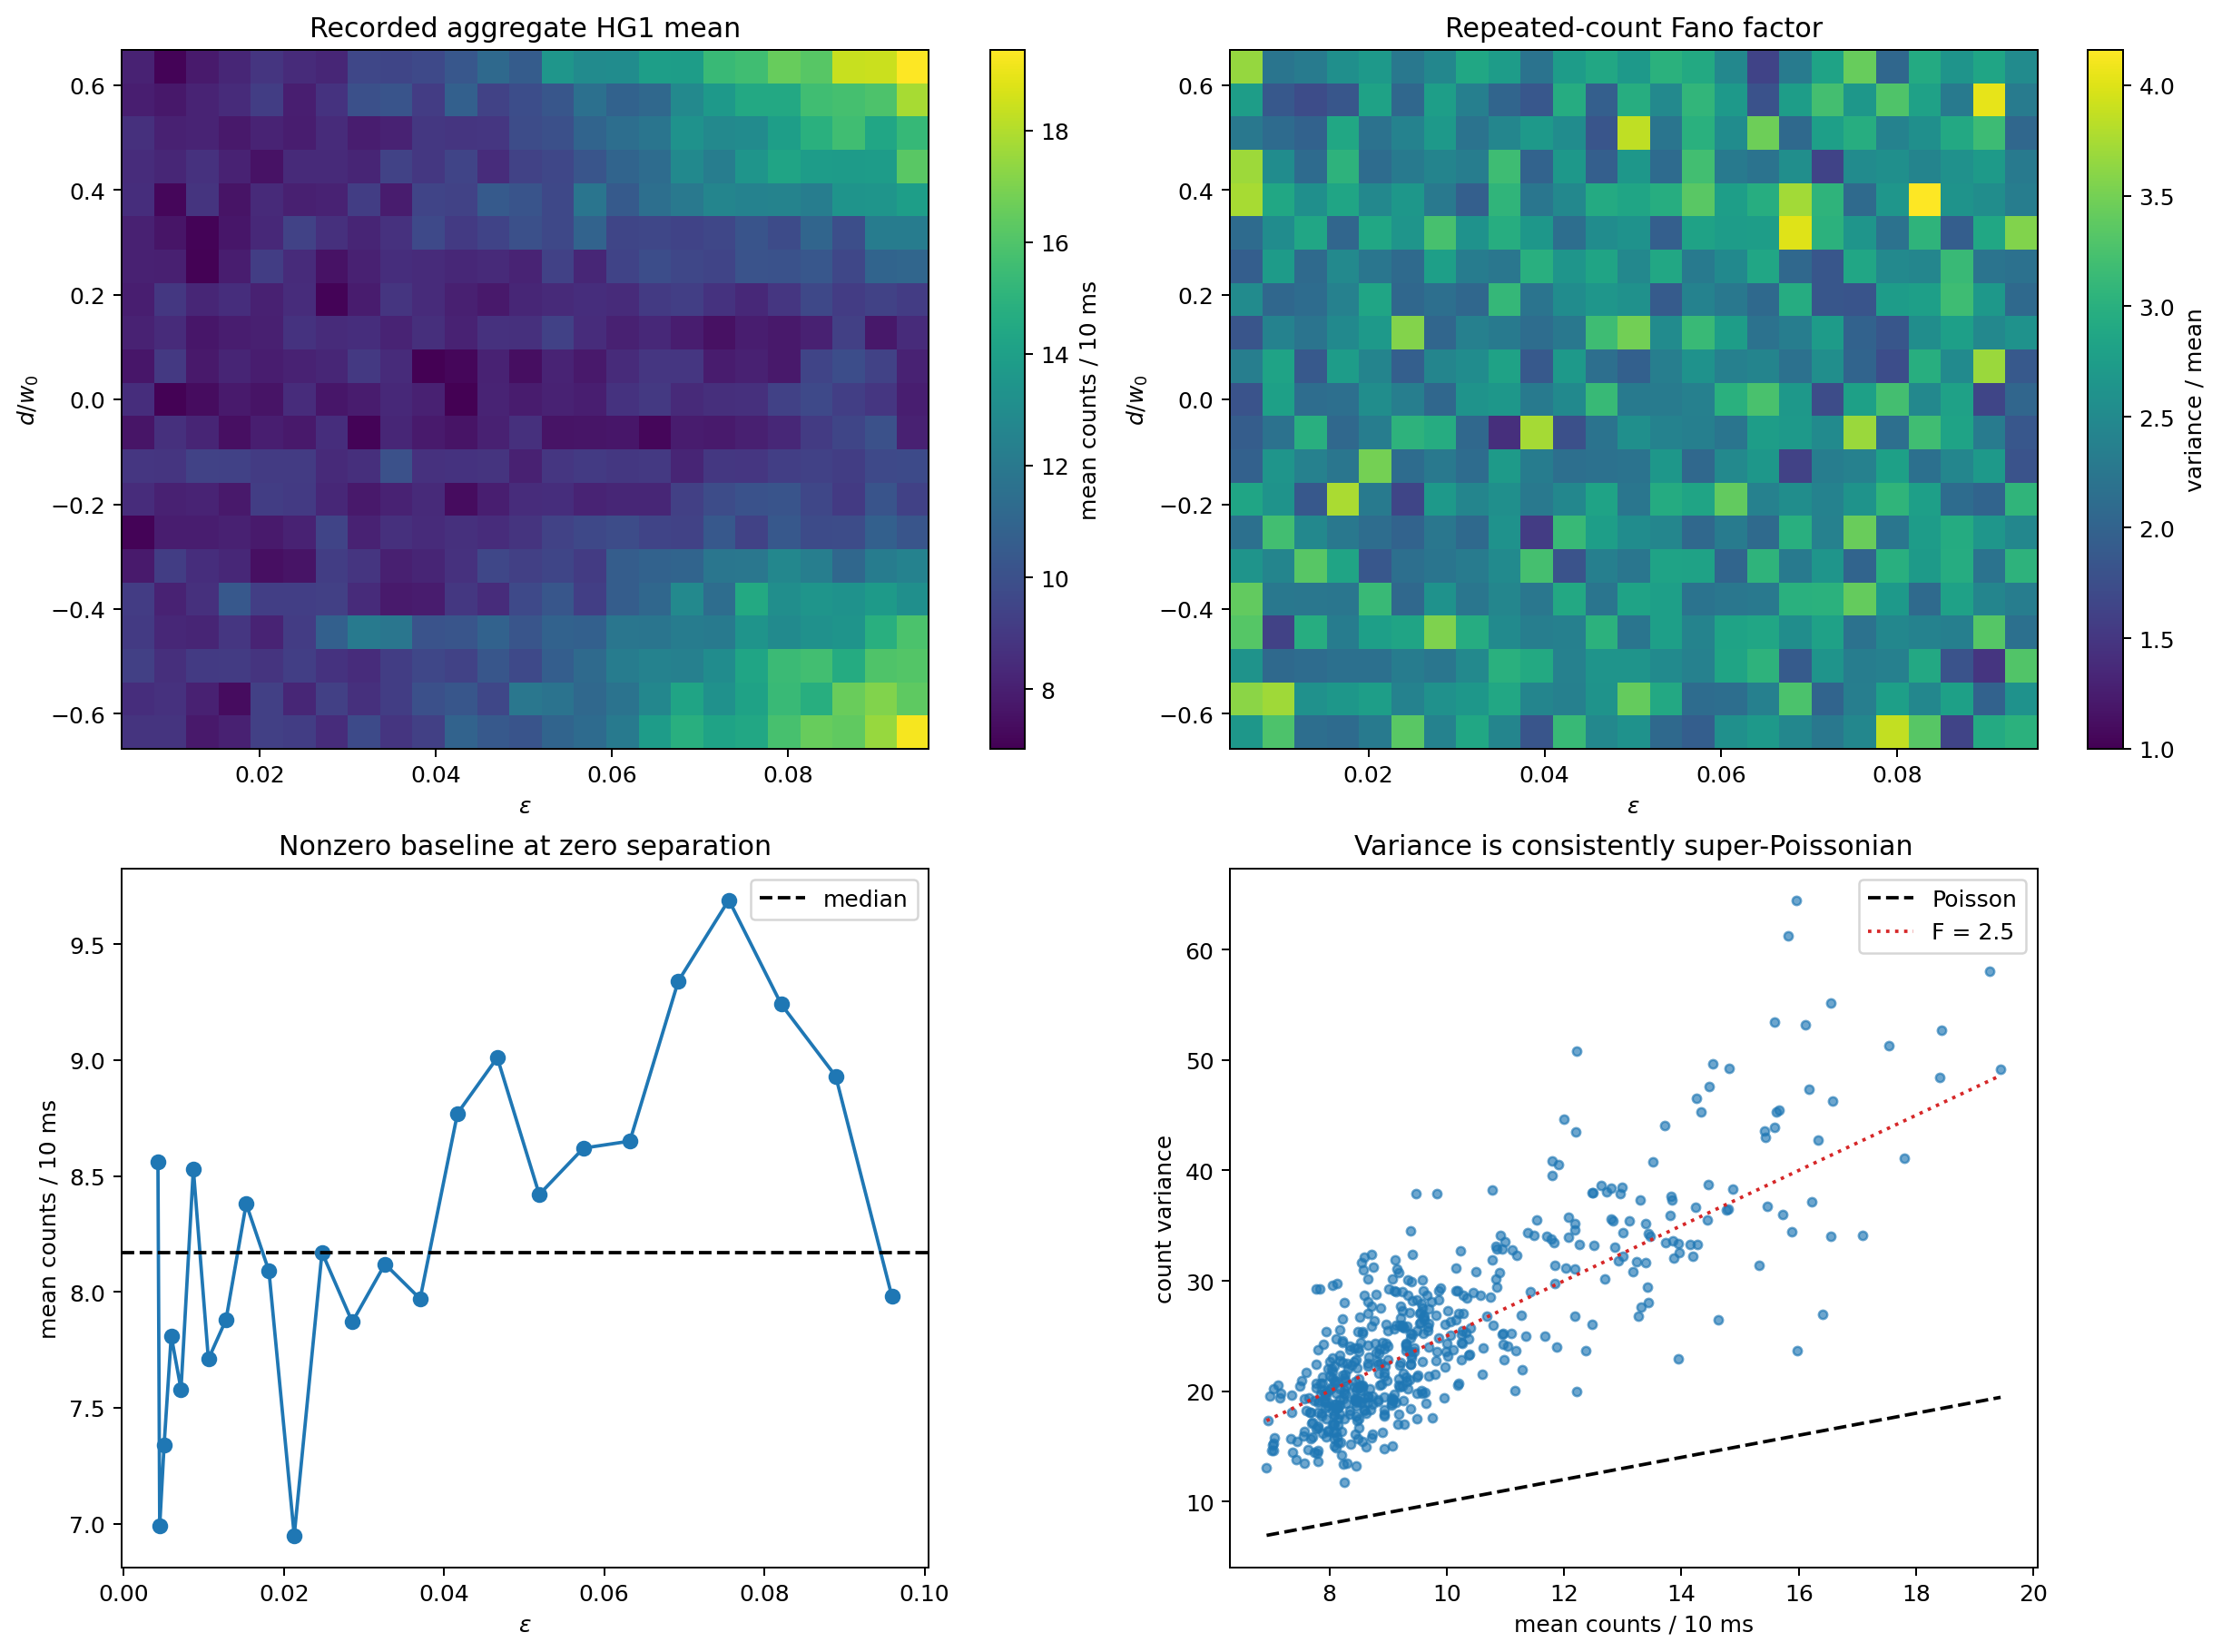
\includegraphics[width=\textwidth]{figures/exoplanets/spade_raw_diagnostics.png}
    \caption{Diagnostics of the recorded $10\,\mathrm{ms}$ aggregate first-order counts.  The panels show setting means, setting-wise Fano factors, the nonzero $d_a=0$ baseline, and variance against mean.  They summarize the $100$ repetitions directly and do not represent predictions from a fitted quantum state.}
    \label{fig:spade_data_record}
\end{figure}

Every stored value is a $10\,\mathrm{ms}$ count.  The paper instead combines the $100$ repetitions and quotes about $40{,}000$--$80{,}000$ detected photons for one second.  The comparable first-order observable is therefore the sum
\begin{equation}
    n_{1,\mathrm{1\,s}}=\sum_{r=1}^{100}n_{1,r}
    \label{eq:spade_one_second_count}
\end{equation}
The median zero-separation aggregate is $817$ counts per second.  The paper-style regression is
\begin{equation}
    n_{1,\mathrm{1\,s}}
    =\chi_{\mathrm{eff}}(\eta n)_{\mathrm{1\,s}}
    +c\epsilon d_a^2
    \label{eq:spade_paper_calibration}
\end{equation}
For the assumed normalization $(\eta n)_{\mathrm{1\,s}}=40{,}000$, the fitted values are
\begin{equation}
    \chi_{\mathrm{eff}}=0.020743\pm0.000109
    \qquad
    c=27{,}282.7\pm430.1
    \qquad R^2=0.88499
    \label{eq:spade_paper_calibration_values}
\end{equation}
For an $80{,}000$ normalization, $c$ is unchanged and $\chi_{\mathrm{eff}}=0.010371\pm0.000054$.  These are effective baseline fractions, not measurements of pure $HG_{00}$-to-$HG_1$ cross-talk.  The paper value $\chi=0.0035$ would contribute only $140$ or $280$ baseline counts at the two one-second normalizations.  Both values are well below the observed offset of about $830$ counts.

\begin{figure}[htbp]
    \centering
    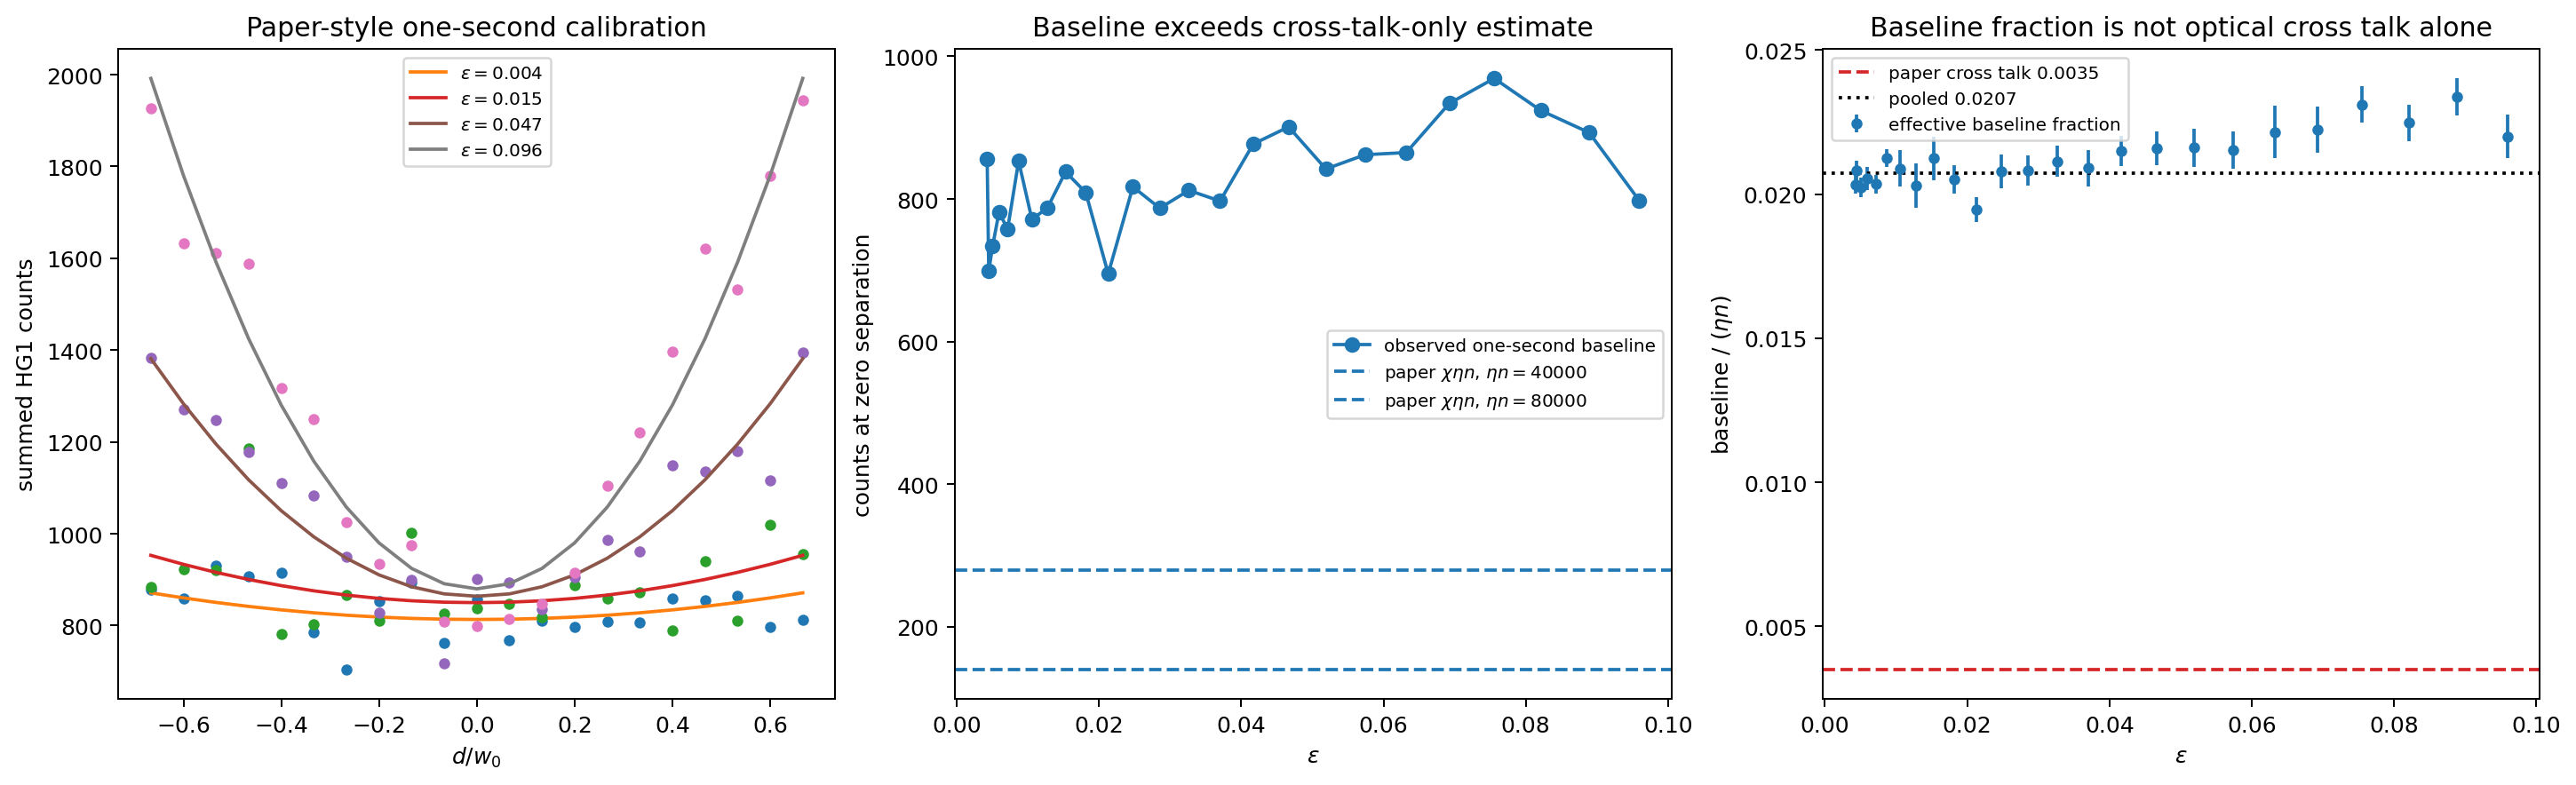
\includegraphics[width=\textwidth]{figures/exoplanets/spade_paper_calibration.png}
    \caption{Paper-style calibration after summing the $100$ independent $10\,\mathrm{ms}$ repetitions at each setting.  The curves and effective baseline fractions are fitted using Eq.~\eqref{eq:spade_paper_calibration}.  The dashed comparison uses the externally reported $\chi=0.0035$.  The fitted baseline is too large to interpret $\chi_{\mathrm{eff}}$ as a measured sorter-transfer probability.}
    \label{fig:spade_paper_calibration}
\end{figure}

The incident-photon, detected-photon, and exposure quantities must remain distinct.  The quantity $N_{\mathrm{in}}$ is the unrecorded number of incident photons in one $10\,\mathrm{ms}$ repetition.  The product $\eta N_{\mathrm{in}}=T$ is the conditional throughput for that repetition.  The paper's $40{,}000$--$80{,}000$ is a one-second detected-photon normalization.  It is neither $N_{\mathrm{in}}$ nor a per-repeat count.

The key exposure point is simple.  Summing the $100$ repetitions gives a one-second total, while averaging them gives a typical $10\,\mathrm{ms}$ count.  These quantities differ by a factor of $100$.

\section{Discrete Counts and Rejected Benchmark Models}

The setting means are only about $7$--$19$ counts, so Gaussian parametric bootstraps can produce non-integer or negative observations.  The following moments define the NB1 diagnostic family.
\begin{equation}
    \operatorname{E}(Y)=\mu
    \qquad
    \operatorname{Var}(Y)=F\mu
    \label{eq:spade_nb1_moments}
\end{equation}
NB1 keeps the observations discrete and uses the factor $F$ to scale the variance above the Poisson value.  The Poisson--lognormal model instead allows the underlying Poisson rate to vary between repetitions.  These models describe two simple forms of overdispersion.

With saturated setting means, NB1 gives $F=2.4188$ and a negative log likelihood of $153{,}969.7$.  The Poisson--lognormal model gives a log-rate standard deviation of $0.3765$ and a negative log likelihood of $153{,}893.2$.  This improves AIC by $153.0$.  The Poisson--lognormal model reproduces the observed number of zero counts, but it still fails checks of variance differences and median skewness within settings.  The two-sided bootstrap $p$-values are $0.00664$ and $0.0133$.  Neither one-parameter family reproduces all the variance and tail structure of the individual counts.

The fixed benchmark uses the illustrative normalization $N_{\mathrm{in}}=40{,}000$ per $10\,\mathrm{ms}$.  It also fixes $\chi=0.0035$, the $HG_1$ transmission at $0.9965$, and $F=2.6$.  Higher-order leakage, background, and offset are set to zero.  The PSF scale and source-ratio exponent are set to one.  The normalization is a scenario assumption, not the paper's one-second detected-photon number.  Within this conditional model,
\begin{equation}
    \begin{aligned}
        \widehat{\eta}=0.0509391
        \qquad &
        \eta\in[0.0505743,0.0513051]
        \\
               & \text{at conditional }99.9\%\text{ profile confidence}
    \end{aligned}
    \label{eq:spade_conditional_eta}
\end{equation}
The observed setting-mean Pearson discrepancy is $4327.62$, compared with a bootstrap median of $524.73$.  For $200$ refitted discrete-count simulations,
\begin{equation}
    p=\frac{1}{201}\simeq0.00498
    \label{eq:spade_fixed_rejection}
\end{equation}
The benchmark is rejected.  Its fitted $\widehat\eta$ is an optimizer within a rejected conditional model, not a measured efficiency.

\begin{figure}[!htb]
    \centering
    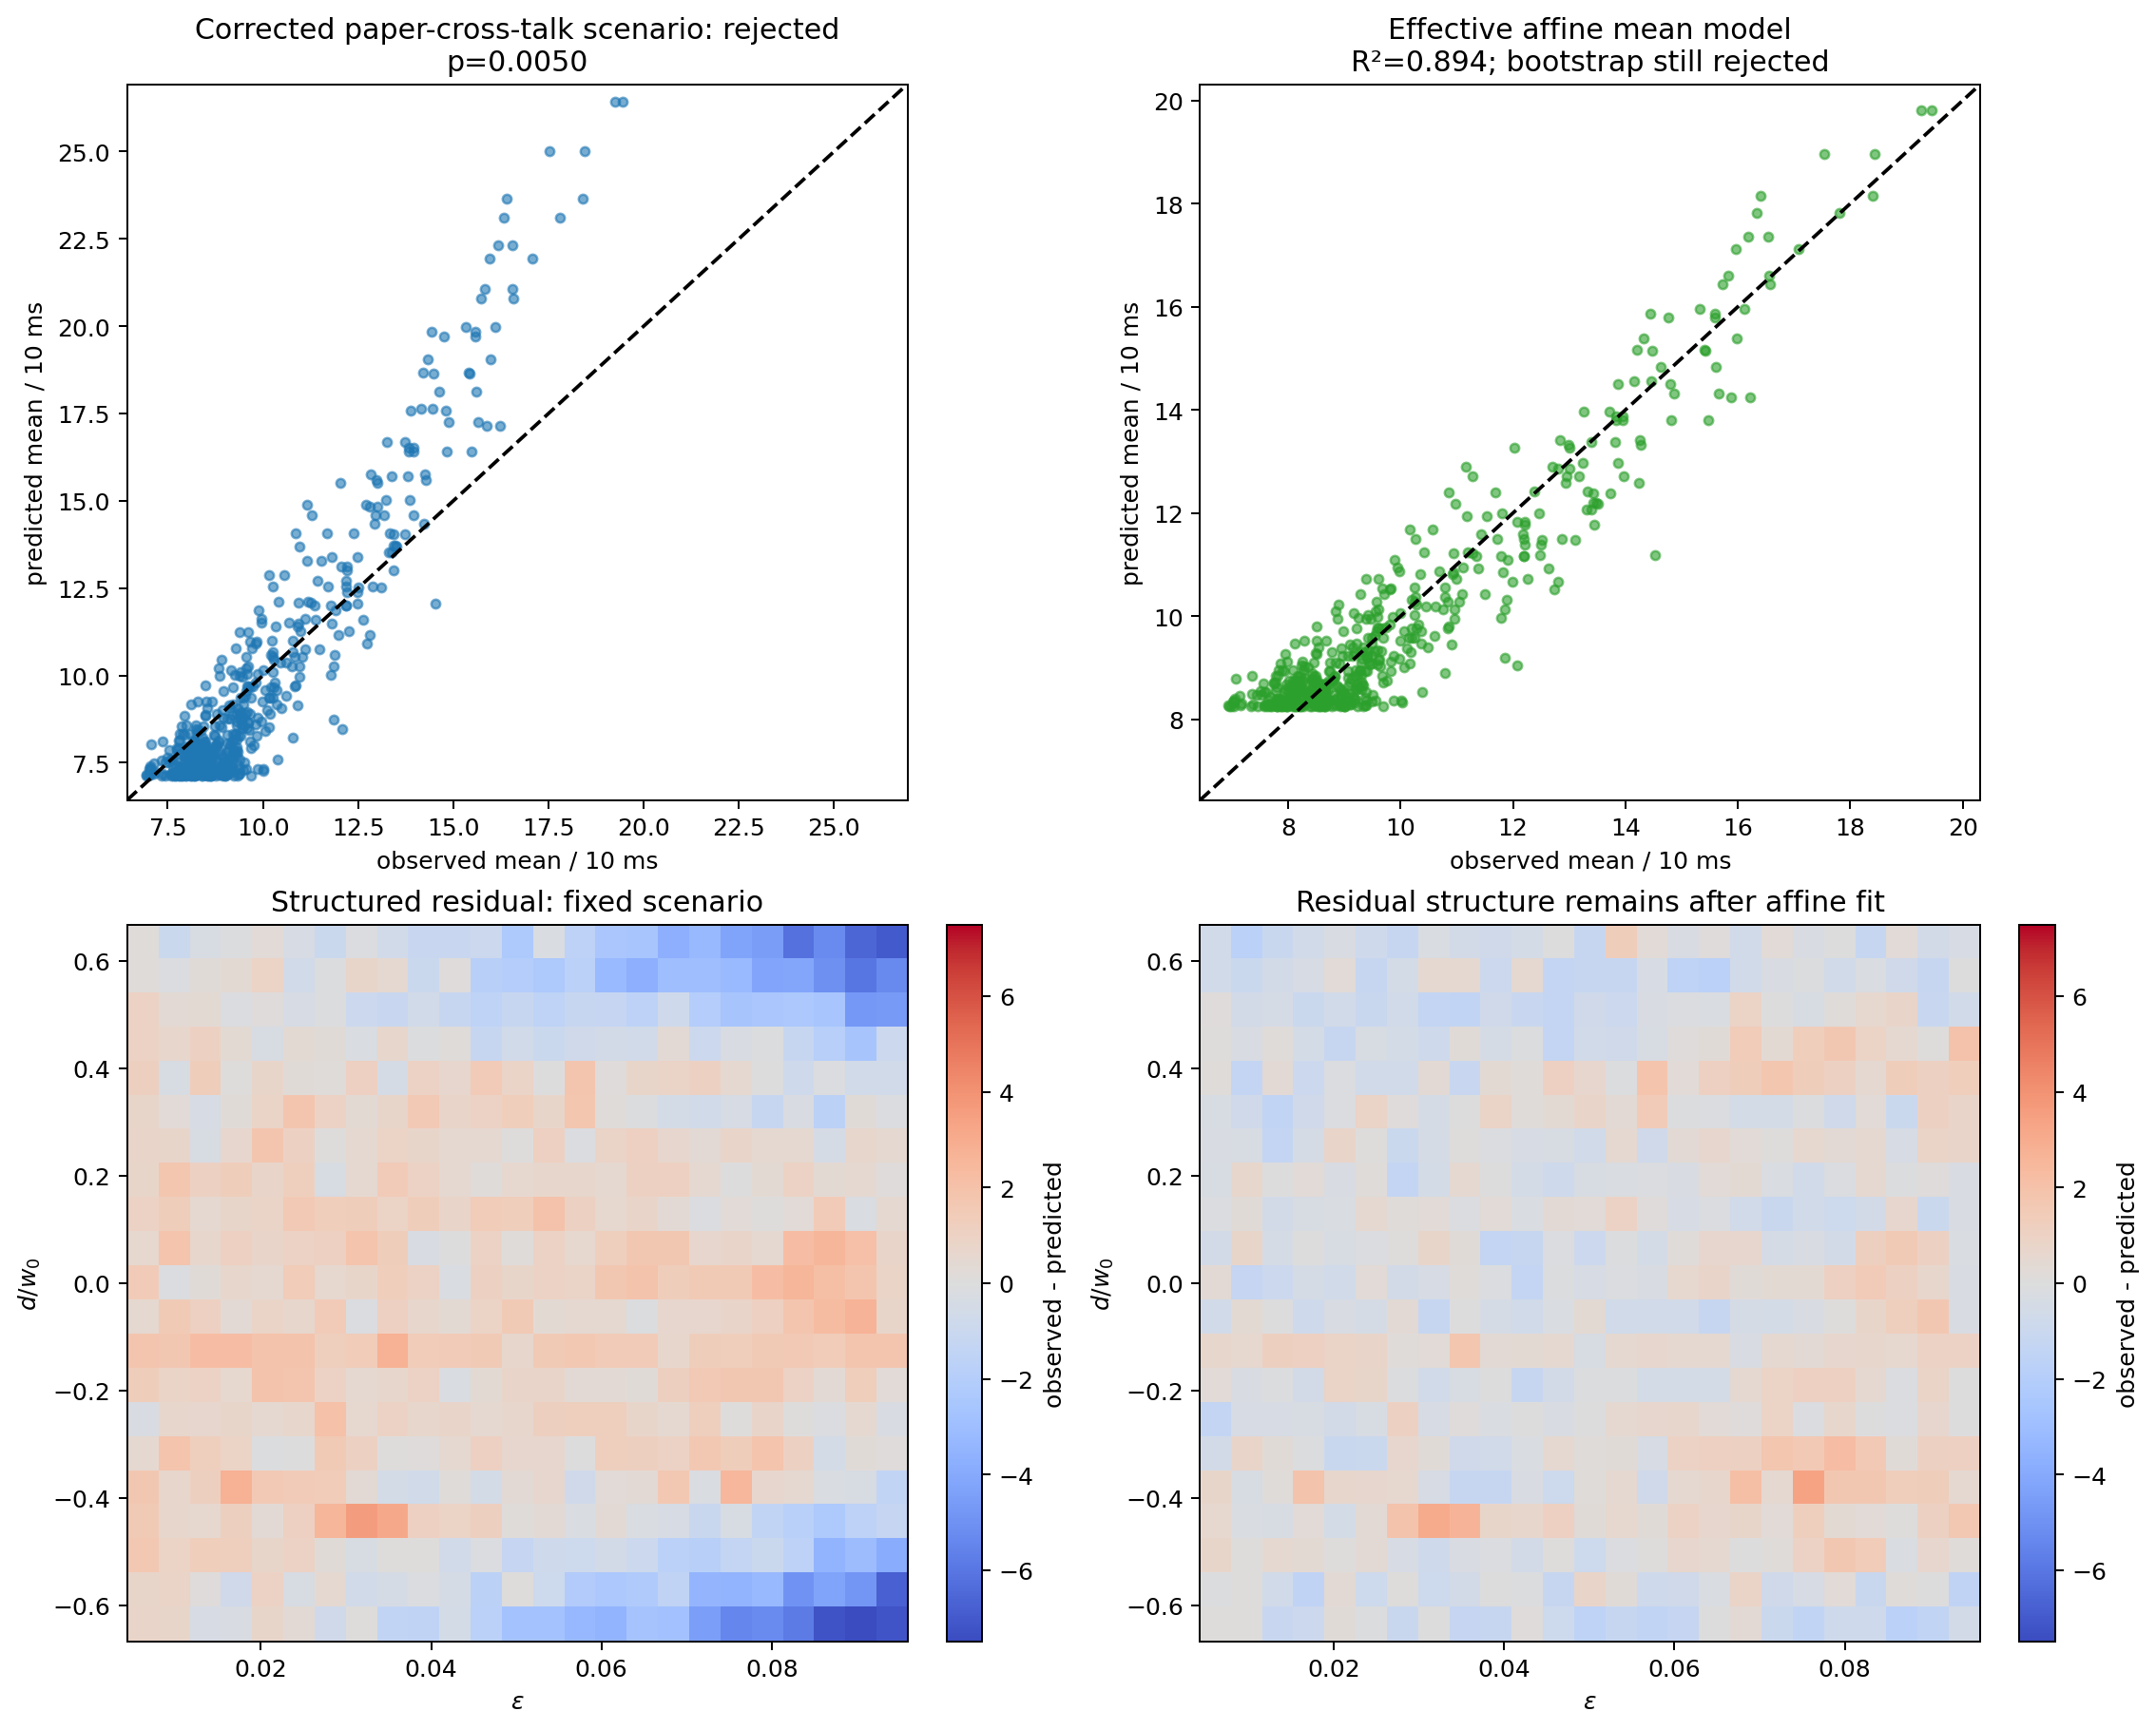
\includegraphics[width=0.92\textwidth]{figures/exoplanets/spade_model_comparison.png}
    \caption{Comparison of the fixed paper-based benchmark channel (left) and an effective affine mean model (right).  Points and residual maps compare fitted and observed $10\,\mathrm{ms}$ setting means.  The discrete bootstrap rejects both models.  Neither panel validates a complete apparatus channel.}
    \label{fig:spade_model_comparison}
\end{figure}

Three more flexible deterministic surfaces were tested with a fitted NB1 Fano factor and a refitted discrete bootstrap.

\begin{table}[htbp]
    \centering
    \caption{Deterministic mean-model diagnostics.  The bootstrap $p$-values use $100$ simulations.}
    \label{tab:spade_explorer_scenarios}
    \begin{tabularx}{\textwidth}{p{3.5cm} c c c c X}
        \toprule
        \textbf{Model}                  & \textbf{$R^2$} & \textbf{$F$} & \textbf{Pearson} & \textbf{$p$} & \textbf{Interpretation}                                 \\
        \midrule
        Affine background + first order & $0.89355$      & $2.4796$     & $1271.1$         & $1/101$      & Useful description, but not a validated data generator  \\
        Source/ calibration deformation & $0.90911$      & $2.4710$     & $1097.7$         & $1/101$      & PSF scale reaches lower bound $0.6$                     \\
        Added higher-order tail         & $0.91650$      & $2.4673$     & $1025.1$         & $1/101$      & Negative tail coefficient absorbs calibration structure \\
        \bottomrule
    \end{tabularx}
\end{table}

The increasing $R^2$ improves the visual fit to the means but does not fix the discrete-count discrepancy.  A PSF scale at its boundary and a negative tail coefficient show that the flexible terms absorb missing calibration structure.  The negative coefficient is not a physical leakage probability.  The standardized repeat average across settings has standard deviation $0.0427$, close to the independent-repeat expectation of $0.0436$.  Its lag-one correlation is $0.044$.  These values give no evidence of a repeat-index drift shared by all settings.  The bootstrap-median Pearson discrepancies are $524.5$, $519.8$, and $523.1$.  They are far below the observed values in Table~\ref{tab:spade_explorer_scenarios}.

\section{Hierarchical Calibration Details}

The central mean and calibration field are defined in Eqs.~\eqref{eq:spade_effective_count_model} and~\eqref{eq:spade_calibration_gp}.  The Gaussian process acts as a smooth calibration correction across the setting grid.  Its amplitude describes the size of the correlated variation, while its length scales describe how quickly that variation changes with displacement and source ratio.

The fit to the full grid gives $B=8.23045$ counts per $10\,\mathrm{ms}$, $A=1225.58$ counts, and $\delta=0.009824$.  The correlated and independent log-response standard deviations are $0.05248$ and $0.02520$.  These correspond to about $5.25\%$ and $2.52\%$.  The correlation lengths are $0.0597w_0$ in displacement and $0.0228$ in $\epsilon$.  The ratio $B/A=0.006716$ is not an optical cross-talk probability unless the background is negligible and the first-order normalization is known independently.

\begin{table}[htbp]
    \centering
    \caption{Grouped five-fold validation of the hierarchical mean channel.  Every fold refits the physical mean, variance law, GP amplitudes, and length scales without the held-out setting means.}
    \label{tab:spade_hierarchical_validation}
    \begin{tabularx}{\textwidth}{Xccc}
        \toprule
        \textbf{Held-out structure}    & \textbf{RMSE} & \textbf{Stand. SD} & \textbf{95\% coverage} \\
        \midrule
        Interleaved checkerboard cells & $0.606$       & $1.004$            & $93.52\%$              \\
        Complete distance rows         & $0.734$       & $1.041$            & $94.67\%$              \\
        Complete source-ratio columns  & $0.609$       & $1.009$            & $93.71\%$              \\
        \bottomrule
    \end{tabularx}
\end{table}

On the full grid, the conditional GP Mahalanobis discrepancy is $527.10$ for about $518$ degrees of freedom.  The value is $p=0.381$ when the hyperparameters are fixed after fitting.  However, the same grid was used to estimate those hyperparameters.  Grouped holdout prediction is therefore the stronger test.

\begin{figure}[htbp]
    \centering
    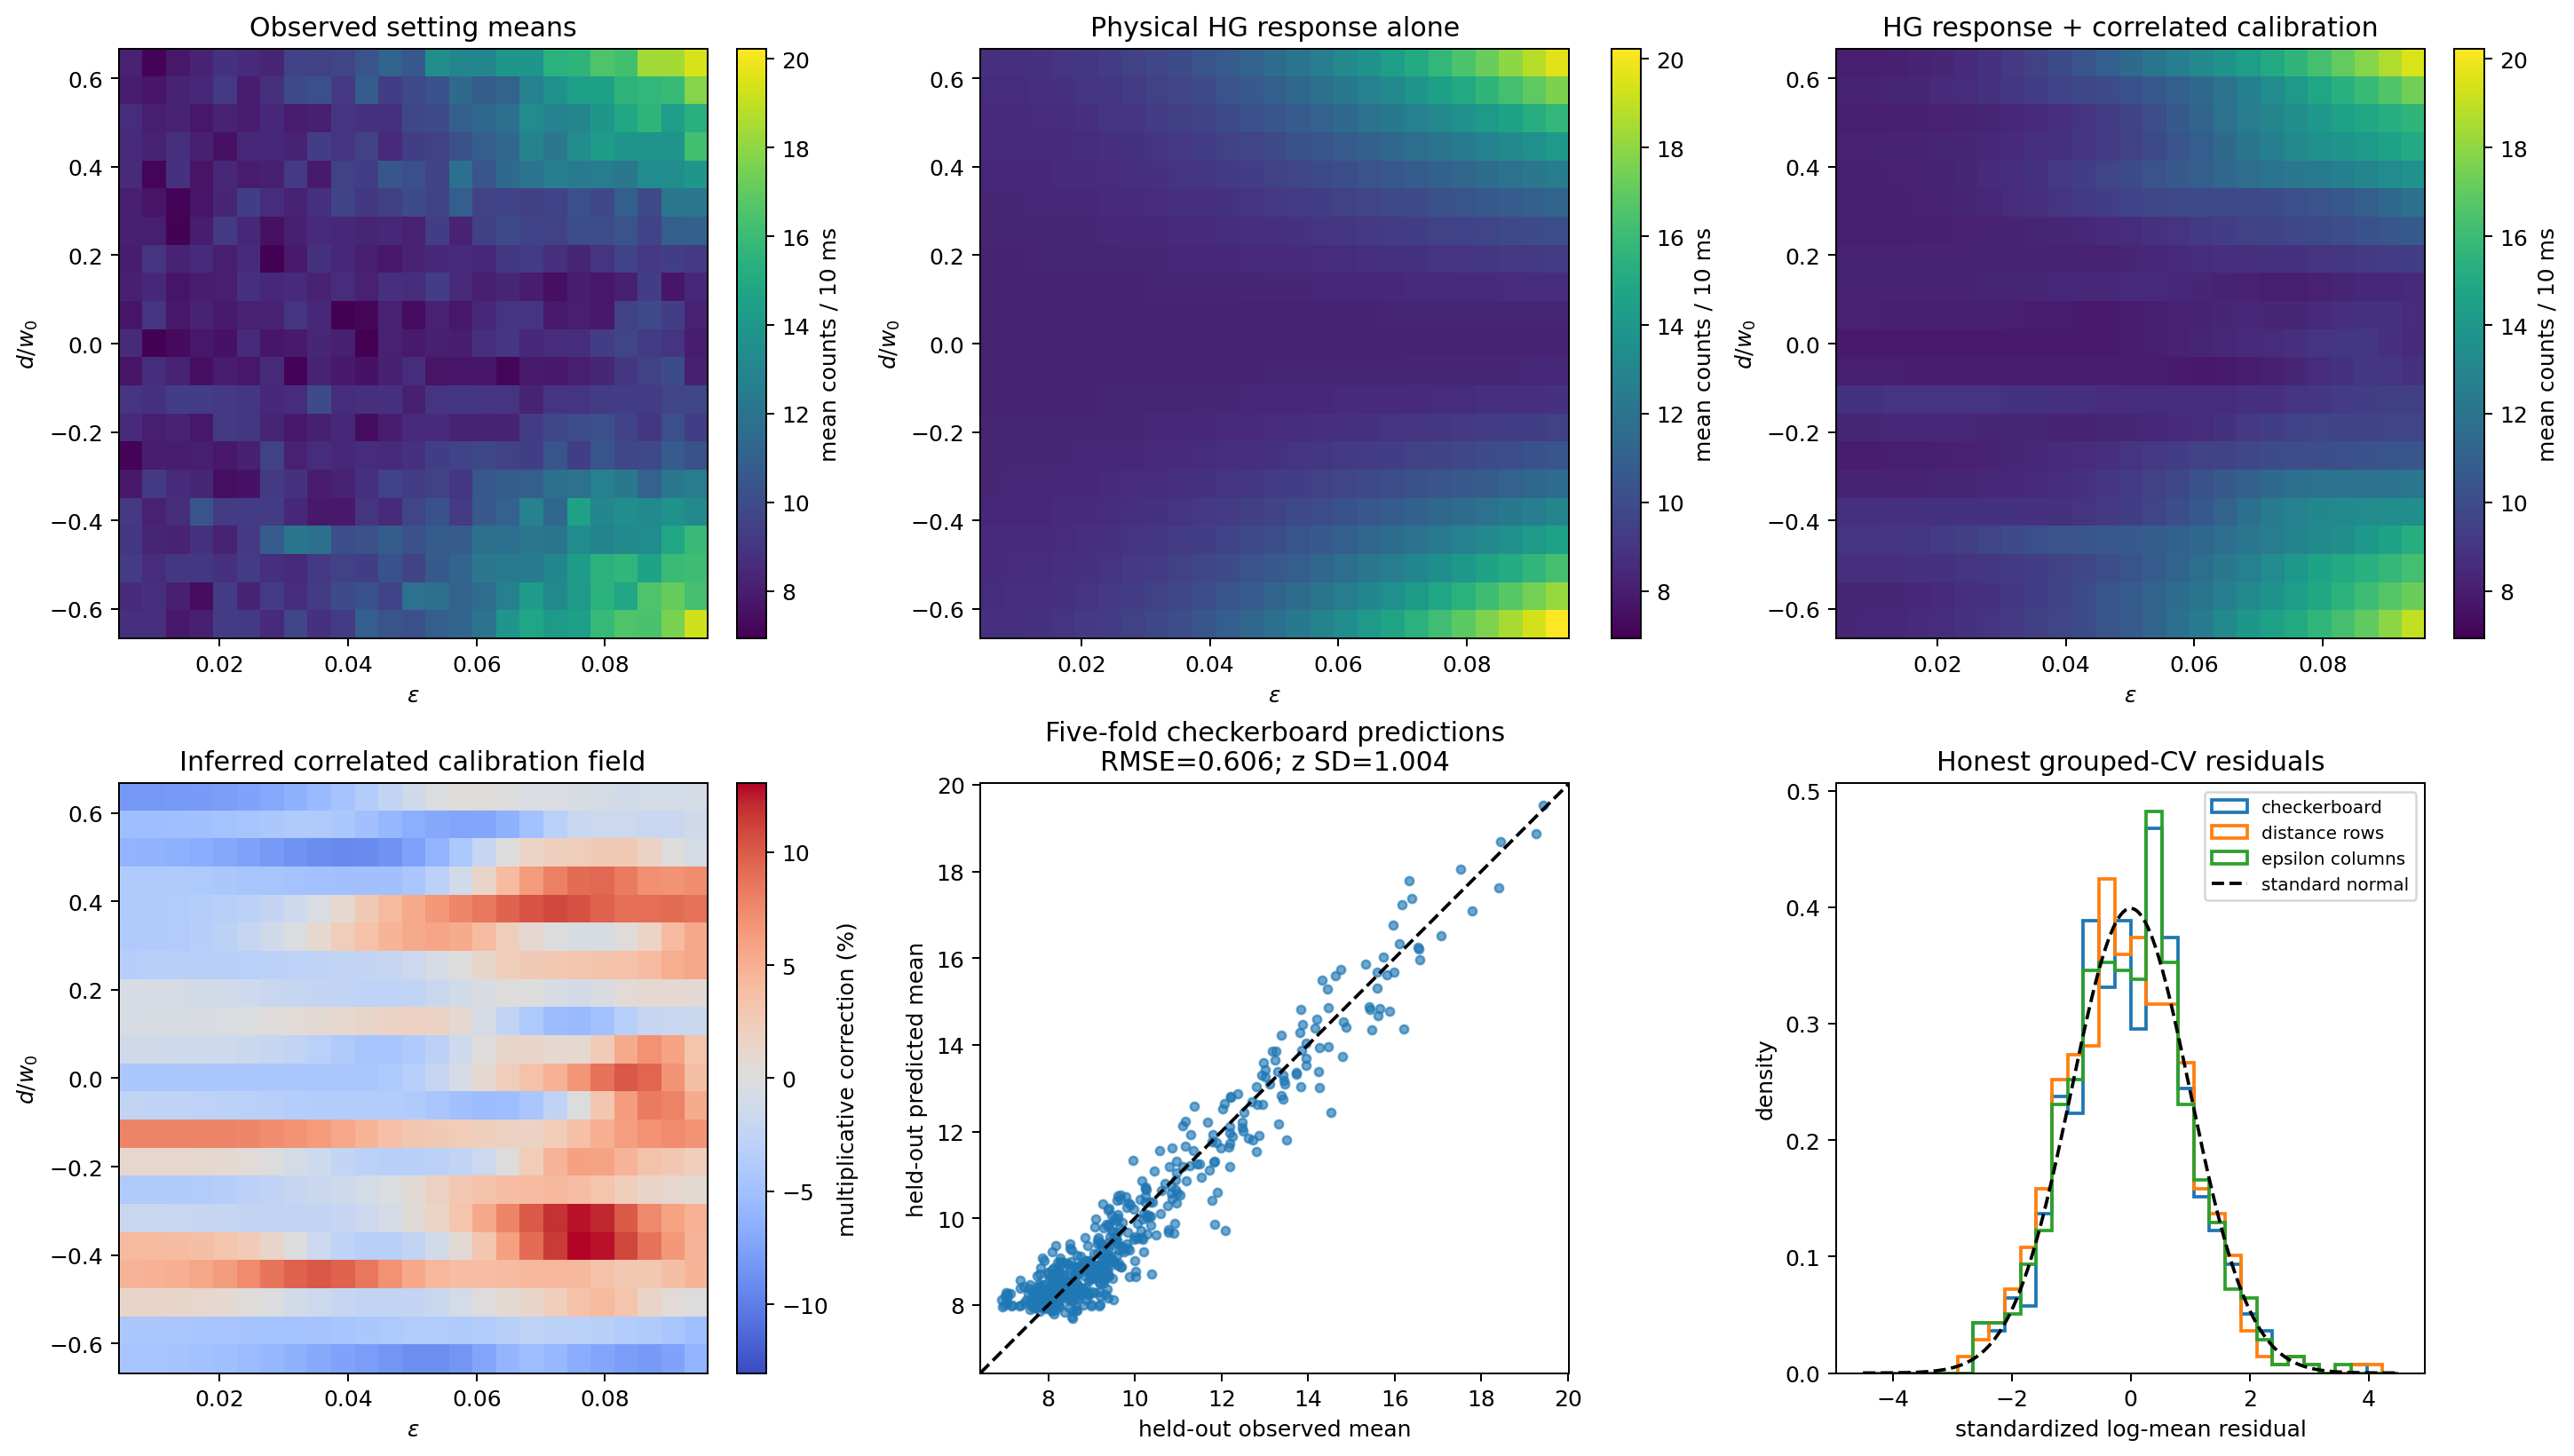
\includegraphics[width=\textwidth]{figures/exoplanets/spade_hierarchical_channel.png}
    \caption{Hierarchical mean channel and grouped holdout validation.  The top row compares observed setting means, the physical center in Eq.~\eqref{eq:spade_effective_count_model}, and the response after the fitted classical calibration field.  The bottom row shows the fitted multiplicative field and held-out predictions.  This validates prediction of the $100$-repeat setting mean, not a complete distribution for each $10\,\mathrm{ms}$ count.}
    \label{fig:spade_hierarchical_channel}
\end{figure}

\section{Identifiable Throughput Details}

The count scale alone cannot show if a larger signal came from more incident photons or from higher survival.  The data therefore identify their product $T=N_{\mathrm{in}}\eta$ more directly than either factor. The fitted response probability is conditional on common survival, so $T$ supplies the survival factor exactly once.

\begin{table}[htbp]
    \centering
    \caption{Identifiable sequential-channel results.  The intervals and envelopes are conditional and do not measure an absolute efficiency.}
    \label{tab:spade_identifiability}
    \begin{tabularx}{\textwidth}{p{5.4cm} p{3.5cm} X}
        \toprule
        \textbf{Quantity}                   & \textbf{Result}                   & \textbf{Status}                                     \\
        \midrule
        Fixed $HG_0/HG_1$ cross-talk $\chi$ & $0.0035$                          & External paper value. Symmetric full matrix assumed \\
        Raw physical-base background        & $3.9099$ counts/$10\,\mathrm{ms}$ & Fitted conditional nuisance                         \\
        Raw physical-base $T$               & $1234.43$ per $10\,\mathrm{ms}$   & Fitted before the calibrated coupling adjustment    \\
        Calibrated $T$                      & $1304.25$ per $10\,\mathrm{ms}$   & Main conditional throughput scale                   \\
        Repeat-resampling 95\% interval     & $[1295.88,1313.06]$               & Conditional on fixed nuisance calibration           \\
        Grouped cross-fit envelope          & $[1251.49,1359.47]$               & Sensitivity to calibration and held-out prediction  \\
        \bottomrule
    \end{tabularx}
\end{table}

The grouped sequential fit gives held-out standardized residual standard deviations of $1.018$, $1.061$, and $1.023$ for checkerboard cells, distance rows, and source-ratio columns.  The corresponding coverages are $93.71\%$, $95.05\%$, and $93.52\%$.  The fitted scale corresponds to $130{,}425$ per second.  This is above the paper's quoted $40{,}000$--$80{,}000$ detected photons per second, but the two quantities have different meanings.  They cannot be equated without the missing flux and modal-throughput metadata.

Changing the assumed $\chi$ from $0$ to $0.0065$ changes the raw throughput only from about $1226$ to $1242$.  Over the same range, the fitted background changes from $8.23$ to $0.16$ counts.  The throughput is fairly stable under this check, but background and cross-talk cannot be identified separately from the aggregate stream.

\section{Provisional Channel Workbench}

The full implementation also provides a sensitivity workbench.  It fixes example values for random displacement, dephasing, coherent mixing, modal loss, and asymmetric readout.  It then fits $T$, background, displacement offset, and a zero-mean coupling field.  The fixed values below were not inferred from the count cube.

\begin{table}[!htb]
    \centering
    \caption{Parameter sources for the provisional workbench.  The shaded row highlights the single externally reported parameter.  All unshaded rows contain invented sensitivity values or assumed symmetries.  They must not be described as measurements.}
    \label{tab:spade_workbench_provenance}
    \begin{tabularx}{\textwidth}{p{4.5cm} p{2.5cm} X}
        \toprule
        \textbf{Parameter}        & \textbf{Value}        & \textbf{Required calibration}                         \\
        \midrule
        Pointing-jitter SD        & $0.01w_0$             & Acquisition-synchronized centroid or alignment series \\
        HG dephasing visibility   & $0.98$                & Phase-sensitive coherent mode tomography              \\
        $HG_0/HG_1$ mixing angle  & $0.01\,\mathrm{rad}$  & Complex mode-injection transfer matrix                \\
        Mixing phase              & $0$                   & Phase-sensitive transfer matrix                       \\
        $HG_0$ transmission       & $0.99$                & Absolute $HG_0$ injection throughput                  \\
        $HG_1$ transmission       & $0.97$                & Separate absolute $HG_{01}$ and $HG_{10}$ throughputs \\
        \rowcolor{gray!20}
        $HG_0\to HG_1$ readout    & $0.0035$              & Repeat the paper's injection calibration              \\
        $HG_1\to HG_0$ readout    & \makecell[l]{$0.0035$                                                         \\ (sym.)}      & Inject first-order modes and record every output      \\
        Failure$\to HG_1$ readout & $0$                   & Inject higher modes and record aggregate $HG_1$       \\
        \bottomrule
    \end{tabularx}
\end{table}

The workbench gives $T=1342.35$ per $10\,\mathrm{ms}$ and a grouped cross-fit envelope of $[1289.62,1399.11]$.  The difference from the main estimate shows how provisional modal loss and mixing can be absorbed into the throughput.

The workbench is modular.  A measured transfer matrix, jitter distribution, or modal transmission can replace the corresponding assumption without changing the inference and QFI pipeline.

Its quantum role comes from the position of these effects in the sequence.  Displacement, dephasing, coherent mixing, and modal loss act on the density operator before the SPADE measurement and can change state QFI or measurement CFI.  Readout confusion acts later on classical probabilities.  The provisional numbers are not what makes the model quantum.

\begin{figure}[!htb]
    \centering
    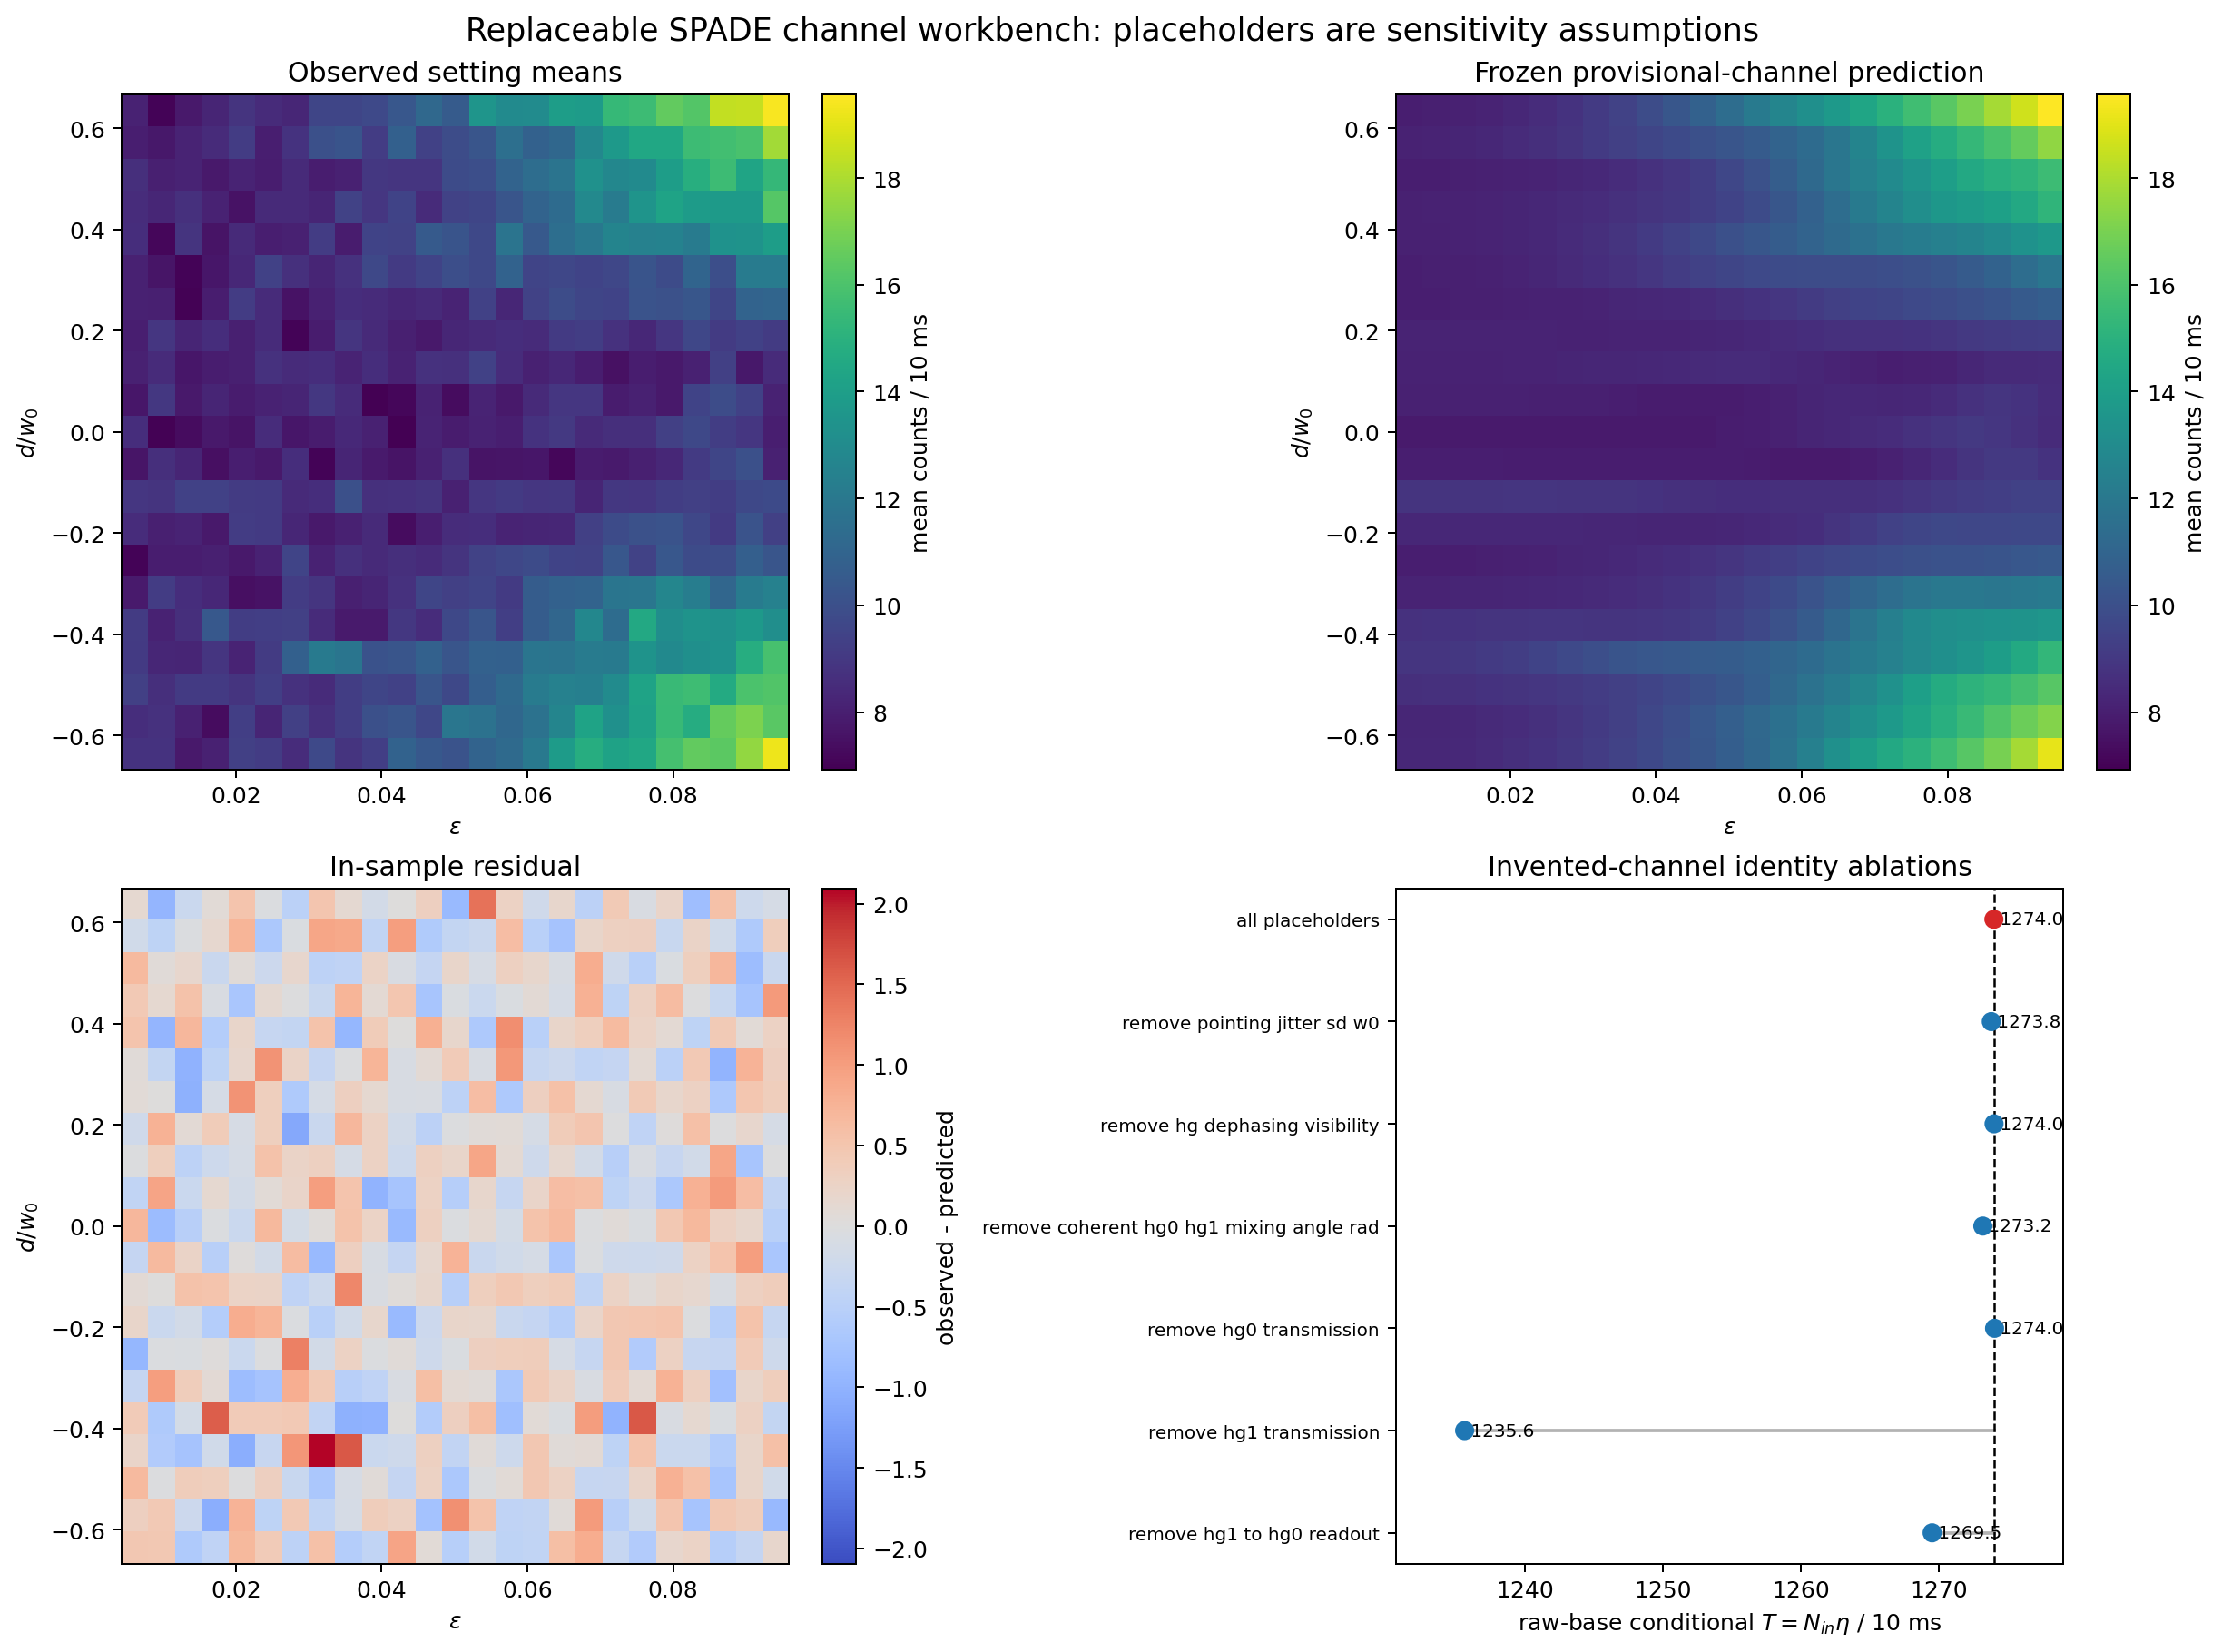
\includegraphics[width=0.92\textwidth]{figures/exoplanets/spade_plausible_channel_workbench.png}
    \caption{Replaceable channel workbench using the provisional values in Table~\ref{tab:spade_workbench_provenance}.  Identity tests show how the inferred throughput depends on individual assumptions.  This is a sensitivity analysis, not an estimate of jitter, dephasing, mixing, transmission, or asymmetric readout.}
    \label{fig:spade_workbench}
\end{figure}
\section{Numerical QFI and CFI Checks}

The ideal source calculation uses the bright-source-aligned convention $\alpha=d_a/2$, an HG basis up to order $12$, and a flagged numerical tail.  At nonzero settings, the maximum relative difference between the SLD and independent finite-fidelity QFI calculations is $0.322\%$.  Increasing the cutoff from order $8$ to order $12$ changes the QFI by at most $5.1\times10^{-12}$ relative.  This small change shows that the finite HG cutoff does not control the reported values.  The point $d_a=0$ is a rank boundary and is excluded from the validation ranges, as explained in Appendix~\ref{app:mathematical_background}.

Table~\ref{tab:spade_information_comparison} gives fractions of source-state QFI for estimating $d_a$, normalized per surviving one-photon trial.  The first two rows use twelve nonzero points from the measured grid.  These points combine three signed distances with four source fractions.  The other rows use a nine-point ladder with $d_a\in\{0.06667,0.4,0.66667\}$ and $\epsilon\in\{0.00427,0.02854,0.09593\}$.

\begin{table}[!htb]
    \centering
    \caption{Theoretical information kept when estimating $d_a$.  All values are fractions of source-state QFI per surviving photon and are conditional model calculations. Shaded rows use the nine-point ladder, unshaded rows use the twelve regular nonzero points from the measured grid.}
    \label{tab:spade_information_comparison}
    \begin{tabularx}{\textwidth}{p{4.8cm} p{1.9cm} X}
        \toprule
        \textbf{Checkpoint}                                    & \textbf{Fraction}      & \textbf{Status} \\
        \midrule
        Full ideal-SPADE CFI                                   & \makecell[l]{$0.99899$                   \\ to $1.00000$} & Theoretical, complete ideal HG outcomes                \\
        \makecell[l]{First-order-only                                                                     \\ binary CFI  }                          & \makecell[l]{$0.78434$                   \\ to $0.94485$} & Theoretical, $HG_1$ versus all other outcomes          \\
        \rowcolor{gray!20}
        \makecell[l]{Flagged $HG_0/HG_1$ accessible-state QFI} & \makecell[l]{$0.99777$                   \\ to $1.00000$} & Theoretical flagged quantum channel                    \\
        \rowcolor{gray!20}
        \makecell[l]{Resolved accessible-outcome CFI}          & \makecell[l]{$0.99681$                   \\ to $1.00000$} & Theoretical measurement of $HG_0$, $HG_1$, and failure \\
        \rowcolor{gray!20}
        \makecell[l]{Binary CFI                                                                           \\ after $\chi=0.0035$ confusion} & \makecell[l]{$0.00134$                \\ to $0.57026$} & Conditional on the assumed symmetric classical readout \\
        \bottomrule
    \end{tabularx}
\end{table}

These calculations are theoretical or conditional.  They do not reconstruct experimental QFI from the aggregate counts.
